\section{模块设计} \label{section: module design}
\subsection{PLL}
PLL是Xilinx的IP核,当用到100MHz以外的时钟频率时可以使用。
在本项目中其配置如图~\ref{fig: pll}。
\begin{figure}[htbp]
    \centering
    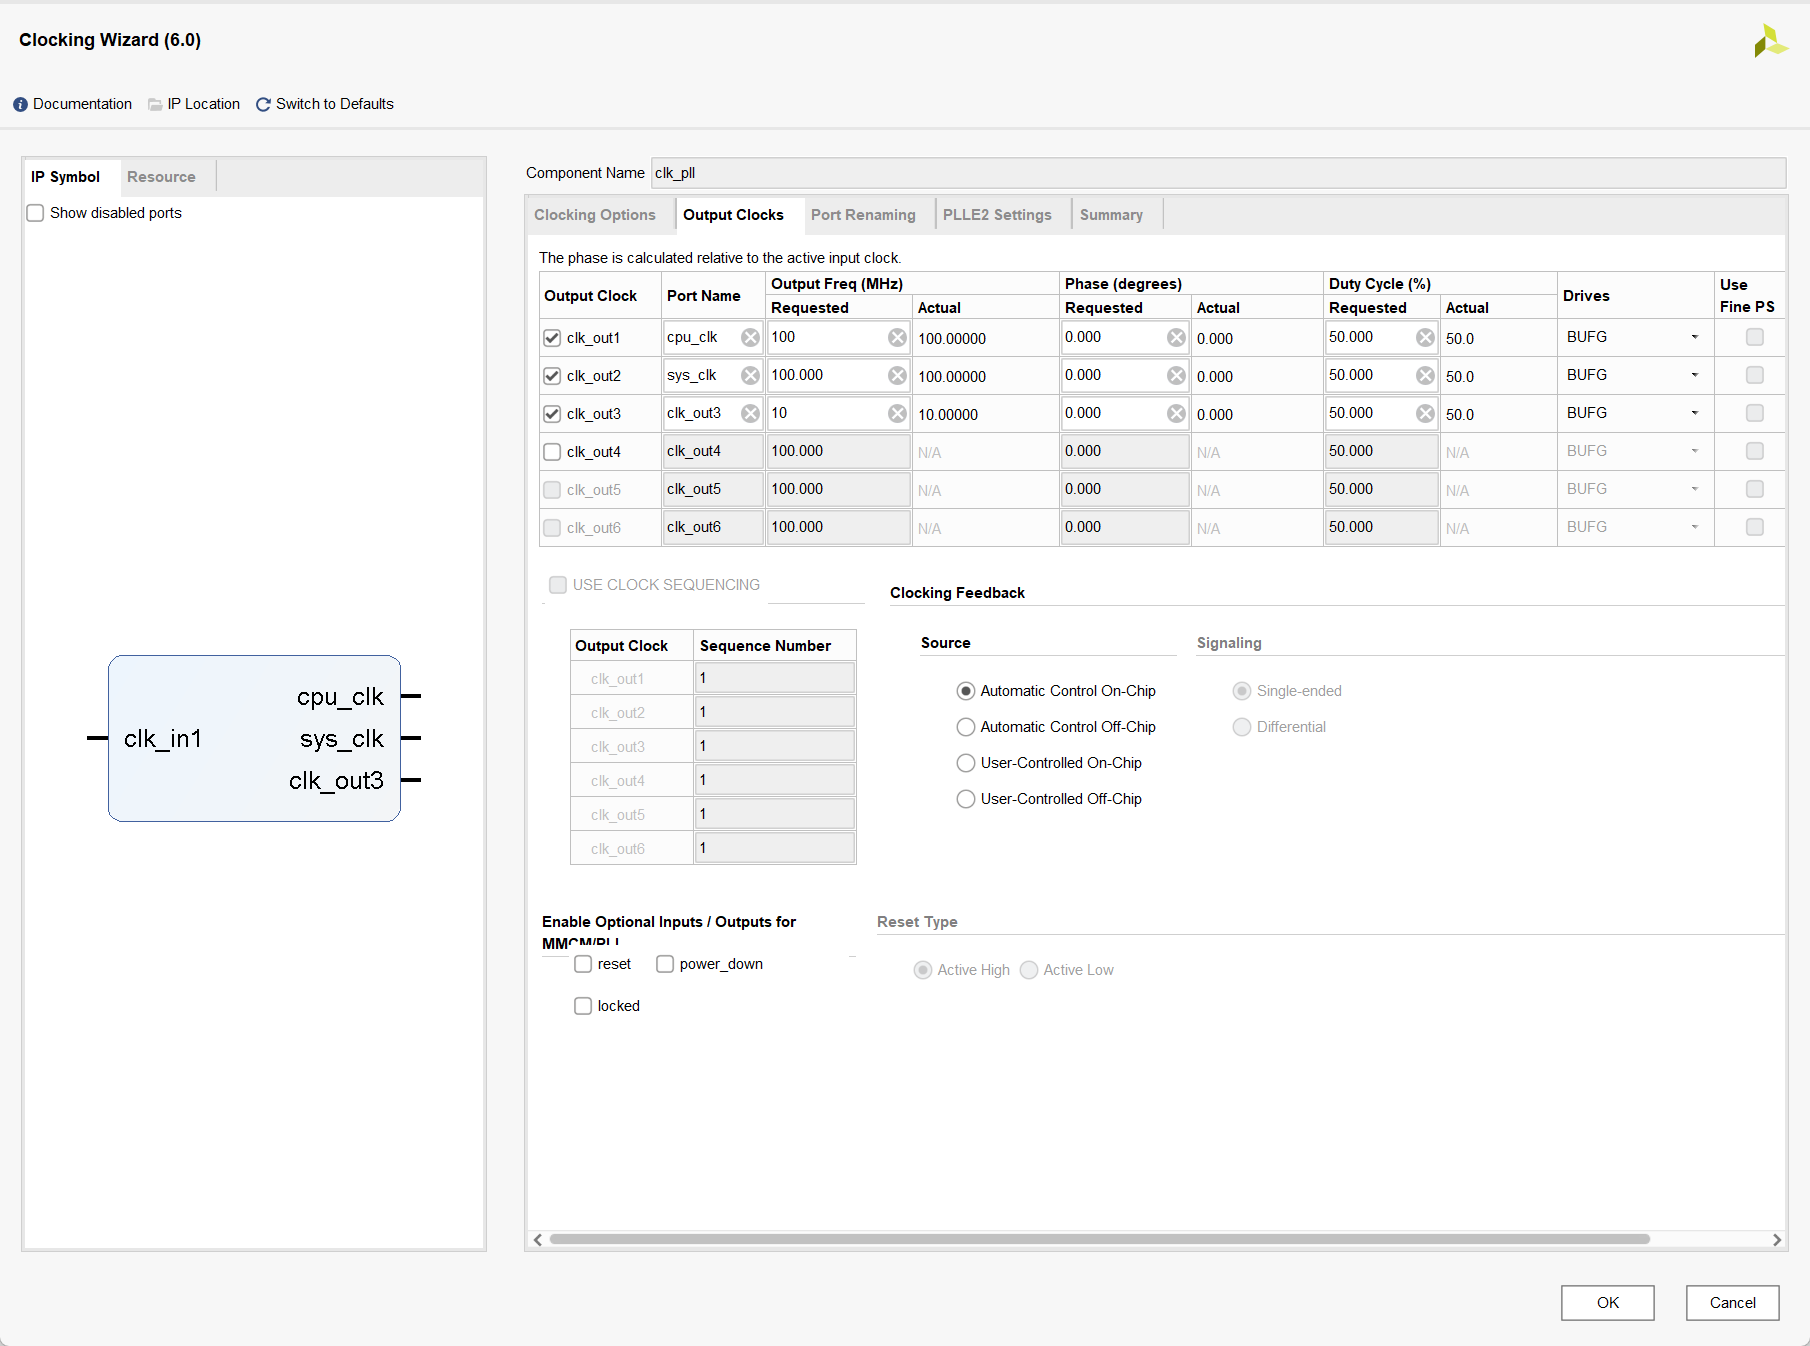
\includegraphics[width=0.7\linewidth]{Figures/1. MyFigs/pll_settings}
    \caption{PLL设置}
    \label{fig: pll}
\end{figure}

\subsection{随机数生成器}
随机数生成器内含一个上电复位为0,不因reset信号重新复位的16位计数器,用于提供伪随机数种子。
每当生成的LED控制信号左右点亮数目相等时,或处于reset后的下一周期时,从该计数器获取随机种。
通过种子不同位的值进行逻辑运算实现随机点亮LED的效果。

\begin{lstlisting}
module random_gen(
        input  wire         clk          ,
        input  wire         take_seed    ,
        output wire [15: 0] random
    );

    reg  [15: 0] random_seed_cnt;
    reg  [15: 0] random_seed;

    always @(posedge clk) begin
        random_seed_cnt <= random_seed_cnt + 'd1;
    end

    always @(posedge clk ) begin
        if(take_seed)
            random_seed <= random_seed_cnt;
    end

    assign random = {
               random_seed[ 0] & random_seed[ 1] ^ random_seed[ 2],
               random_seed[ 3] & random_seed[ 4] ^ random_seed[ 5],
               random_seed[ 6] & random_seed[ 7] ^ random_seed[ 8],
               random_seed[ 9] & random_seed[10] ^ random_seed[11],
               random_seed[12] & random_seed[13] ^ random_seed[14],
               random_seed[15] & random_seed[ 0] ^ random_seed[ 1],
               random_seed[ 2] & random_seed[ 3] ^ random_seed[ 4],
               random_seed[ 5] & random_seed[ 6] ^ random_seed[ 7],
               random_seed[ 8] & random_seed[ 9] ^ random_seed[10],
               random_seed[11] & random_seed[12] ^ random_seed[13],
               random_seed[14] & random_seed[15] ^ random_seed[ 0],
               random_seed[ 1] & random_seed[ 2] ^ random_seed[ 3],
               random_seed[ 4] & random_seed[ 5] ^ random_seed[ 6],
               random_seed[ 7] & random_seed[ 8] ^ random_seed[ 9],
               random_seed[10] & random_seed[11] ^ random_seed[12],
               random_seed[13] & random_seed[14] ^ random_seed[15]
           };
endmodule

\end{lstlisting}

\subsection{状态机}
如图~\ref{fig: fsm}~所示(复位信号已省略),当进入START状态时,等待1s计时结束。
随后进入READY状态,生成LED控制信号直到两侧点亮数量不等为止。
COUNT阶段显示当前用时,直到检测到正确的按键信号传来跳转到ENDD,或者超时跳转到FAIL。
到达ENDD和FAIL状态后等待下一次复位信号重置状态机。

\begin{lstlisting}
parameter    IDLE  = 8'b0000_0001,
             START = 8'b0000_0010,
             READY = 8'b0000_0100,
             COUNT = 8'b0000_1000,
             ENDD  = 8'b0001_0000,
             FAIL  = 8'b0010_0000;

always @(posedge sys_clk) begin
        if(rst)
            current_state <= IDLE;
        else
            current_state <= next_state;
    end

    always @(*) begin
        if(rst)
            next_state = IDLE;
        else
        case (current_state)
            IDLE :
                next_state = START;
            START :
                next_state = stop ? READY : START;
            READY :
                next_state = ~stop & ~equal ? COUNT : READY;
            COUNT :
                next_state = stop ? FAIL : correct ? ENDD : COUNT;
            ENDD :
                next_state = ENDD;
            FAIL :
                next_state = FAIL;
            default:
                next_state = IDLE;
        endcase
    end

\end{lstlisting}

\begin{figure}[htbp]
    \centering
    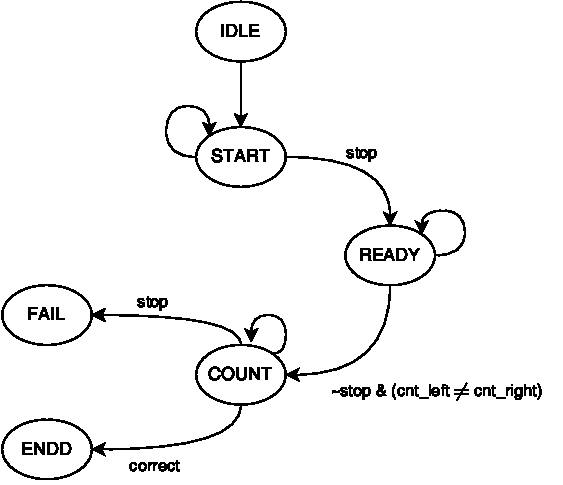
\includegraphics[width=0.5\linewidth]{Figures/1. MyFigs/fsm}
    \caption{状态机图}
    \label{fig: fsm}
\end{figure}

\subsection{按键消抖模块}
通过接入较为低频的时钟信号减少此处计数器的位宽,当按键输入为高电平时累计计数器,
当按键输入为低时立刻将计数器置0。在计数器累计为指定值后若按键输入依然为高则保持计数器不变。

当计数器为指定值时输出高电平,表示该按键消抖后的信号。

\begin{lstlisting}
reg  [ 3: 0] cnt [ 3: 0];

genvar i;
generate
    for (i = 0; i < 4; i = i + 1) begin
        always @(posedge clk ) begin
            if(key_col_i[i] & (cnt[i]!='hF))
                cnt[i] <= cnt[i] + 'd1;
            else if(key_col_i[i] & cnt[i]=='hF)
                cnt[i] <= cnt[i];
            else
                cnt[i] <= 'b0;
        end

        assign key_col_o[i] = (cnt[i]=='hF);
    end
endgenerate
\end{lstlisting}

\subsection{判断器}
该模块通过接收LED控制信号从而计算两侧1的数量,并指示哪一侧的0(LED低电平点亮)数量更多并输出。
\begin{lstlisting}
module judger (
        input  wire         clk       ,
        input  wire         rst       ,
        input  wire [15: 0] ans_i     ,
        input  wire [ 3: 0] key_i     ,
        input  wire         ready     ,
        output wire         equal     ,
        output reg          correct   ,
        output wire         is_correct
    );

    wire [ 3: 0] cnt_left  ;
    wire [ 3: 0] cnt_right ;

    assign cnt_left =
           ans_i[ 0] +
           ans_i[ 1] +
           ans_i[ 2] +
           ans_i[ 3] +
           ans_i[ 4] +
           ans_i[ 5] +
           ans_i[ 6] +
           ans_i[ 7] ;

    assign cnt_right =
           ans_i[ 8] +
           ans_i[ 9] +
           ans_i[10] +
           ans_i[11] +
           ans_i[12] +
           ans_i[13] +
           ans_i[14] +
           ans_i[15] ;

    assign is_correct =
           ready & |key_i[1:0] & ~|key_i[3:2] & (cnt_left > cnt_right) |
           ready & |key_i[3:2] & ~|key_i[1:0] & (cnt_left < cnt_right);

    assign equal = (cnt_left == cnt_right);

    always @(posedge clk ) begin
        if(rst)
            correct <= 'b0;
        else if(is_correct)
            correct <= 'b1;
    end

endmodule
\end{lstlisting}


\subsection{十进制计数器}
十进制计数器当READY状态或reset信号到来时清零,并每当累积到9后与上一级时钟信号相与
产生下一级的时钟信号,并将当前级清零。

\begin{lstlisting}
module counter (
        input  wire         clk      ,
        input  wire         clk_10MHz,
        input  wire         rst      ,
        input  wire         stop     ,
        input  wire         fsm_ready,
        output reg  [15: 0] data     ,
        output wire         clk_seg  ,
        output wire         clk_10kHz
    );

    reg  [15: 0] cnt;
    reg  [ 9: 0] cnt_10kHz ;

    wire         clk_1kHz  ;
    wire         clk_100Hz ;
    wire         clk_10Hz  ;

    assign clk_10kHz = (cnt_10kHz == 'd999);
    assign clk_1kHz = (data[0+:4]=='h9) & clk_10kHz;
    assign clk_100Hz = (data[4+:4]=='h9) & clk_1kHz;
    assign clk_10Hz = (data[8+:4]=='h9) & clk_100Hz;
    assign clk_seg = cnt[15];

    always @(posedge clk ) begin
        if(clk_seg)
            cnt <= 'd0;
        else
            cnt <= cnt + 'd1;
    end

    always @(posedge clk_10MHz) begin
        if(rst | clk_10kHz)
            cnt_10kHz <= 'd0;
        else
            cnt_10kHz <= cnt_10kHz + 'd1;
    end

    always @(posedge clk_10MHz ) begin
        if(rst | clk_1kHz & ~stop | fsm_ready)
            data[0+:4] <= 'd0;
        else if(stop)
            data[0+:4] <= data[0+:4];
        else if(clk_10kHz)
            data[0+:4] <= data[0+:4] + 'd1;
    end

    always @(posedge clk_10MHz ) begin
        if(rst | clk_100Hz & ~stop | fsm_ready)
            data[4+:4] <= 'd0;
        else if(stop)
            data[4+:4] <= data[4+:4];
        else if(clk_1kHz)
            data[4+:4] <= data[4+:4] + 'd1;
    end

    always @(posedge clk_10MHz ) begin
        if(rst | clk_10Hz & ~stop | fsm_ready)
            data[8+:4] <= 'd0;
        else if(stop)
            data[8+:4] <= data[8+:4];
        else if(clk_100Hz)
            data[8+:4] <= data[8+:4] + 'd1;
    end

    always @(posedge clk_10MHz ) begin
        if(rst | fsm_ready)
            data[12+:4] <= 'd0;
        else if(stop)
            data[12+:4] <= data[12+:4];
        else if(clk_10Hz)
            data[12+:4] <= data[12+:4] + 'd1;
    end

endmodule
\end{lstlisting}

\subsection{数码管控制}
数码管控制使用分频器引出的数码管控制时钟,利用八进制计数器控制片选信号,轮流使能数码管,
并将相应的数据位赋值给数码管的控制信号。

\begin{lstlisting}
module data2seg (
    input  wire         clk    ,
    input  wire [ 3: 0] data   ,
    output reg  [ 6: 0] seg_num
);

always @(posedge clk ) begin
    case (data)
        4'h0:
            seg_num <= 'b1111_110;
        4'h1:
            seg_num <= 'b0110_000;
        4'h2:
            seg_num <= 'b1101_101;
        4'h3:
            seg_num <= 'b1111_001;
        4'h4:
            seg_num <= 'b0110_011;
        4'h5:
            seg_num <= 'b1011_011;
        4'h6:
            seg_num <= 'b1011_111;
        4'h7:
            seg_num <= 'b1110_000;
        4'h8:
            seg_num <= 'b1111_111;
        4'h9:
            seg_num <= 'b1111_011;
        4'hA:
            seg_num <= 'b1110_111;
        4'hB:
            seg_num <= 'b0011_111;
        4'hC:
            seg_num <= 'b1001_110;
        4'hD:
            seg_num <= 'b0111_101;
        4'hE:
            seg_num <= 'b1001_111;
        4'hF:
            seg_num <= 'b1000_111;
    endcase
end

endmodule

reg  [ 3: 0] data_in;

always @(posedge clk) begin
    if(rst)
        seg_csn <= 'b0000_0000;
    else if(seg_csn[7])
        seg_csn <= {seg_csn[6:0], 1'b1};
    else
        seg_csn <= 'b1111_1110;
end

always @(posedge clk ) begin
    if(rst) begin
        data_in <= 'h0;
    end
    else begin
        case (seg_csn)
            8'b1111_1110:
                data_in <= data[ 0+:4];
            8'b1111_1101:
                data_in <= data[ 4+:4];
            8'b1111_1011:
                data_in <= data[ 8+:4];
            8'b1111_0111:
                data_in <= data[12+:4];
            8'b1110_1111:
                data_in <= data[16+:4];
            8'b1101_1111:
                data_in <= data[20+:4];
            8'b1011_1111:
                data_in <= data[24+:4];
            8'b0111_1111:
                data_in <= data[28+:4];
            default:
                data_in <= 'h0;
        endcase
    end
end

data2seg u_data2seg(
             //ports
             .clk     		( clk        ),
             .data    		( data_in    ),
             .seg_num 		( seg_num    )
         );
\end{lstlisting}